% Define the top matter
\setModuleTitle{\textit{de novo} Genome Assembly}
\setModuleAuthors{%
  Matthias Haimel \mailto{mhaimel@ebi.ac.uk}\\
  Nathan S. Watson-Haigh \mailto{nathan.watson-haigh@awri.com.au}
}
\setModuleContributions{%
  
}

%  Start: Module Title Page
\chapter{\moduleTitle}
\newpage
% End: Module Title Page

\section{Key Learning Outcomes}

After completing this practical the trainee should be able to:
\begin{itemize}
  \item Compile velvet with appropriate compile-time parameters set for a specific analysis
  \item Be able to choose appropriate assembly parameters
  \item Assemble a set of single-ended reads
  \item Assemble a set of paired-end reads from a single insert-size library
%  \item Assemble a set of long 454 single-end reads
%  \item Assemble multiple paired-end libraries with different insert-sizes
%  \item Assemble a hybrid set of long 454 single-end reads and a set of paired-end reads
  \item Be able to visualise an assembly in AMOS Hawkeye
  \item Understand the importance of using paired-end libraries in \textit{de
        novo} genome assembly
\end{itemize}

\section{Resources You'll be Using}
Although we have provided you with an environment which contains all the tools
and data you will be using in this module, you may like to know where we have
sourced those tools and data from.
 
\subsection{Tools Used}
\begin{description}[style=multiline,labelindent=0cm,align=left,leftmargin=1cm]
  \item[Velvet] \hfill\\
  	\url{http://www.ebi.ac.uk/~zerbino/velvet/}
  \item[AMOS Hawkeye] \hfill\\
    \url{http://apps.sourceforge.net/mediawiki/amos/index.php?title=Hawkeye}
  \item[gnx-tools] \hfill\\
    \url{https://github.com/mh11/gnx-tools}
  \item[FastQC] \hfill\\
    \url{http://www.bioinformatics.bbsrc.ac.uk/projects/fastqc/}
  \item[R] \hfill\\
    \url{http://www.r-project.org/}
\end{description}

\subsection{Sources of Data}
\begin{itemize}
\item \url{ftp://ftp.ensemblgenomes.org/pub/release-8/bacteria/fasta/Staphylococcus/s_aureus_mrsa252/dna/s_aureus_mrsa252.EB1_s_aureus_mrsa252.dna.chromosome.Chromosome.fa.gz}
% single end data
\item \url{http://www.ebi.ac.uk/ena/data/view/SRS004748}
\item \url{ftp://ftp.sra.ebi.ac.uk/vol1/fastq/SRR022/SRR022825/SRR022825.fastq.gz}
\item \url{ftp://ftp.sra.ebi.ac.uk/vol1/fastq/SRR022/SRR022823/SRR022823.fastq.gz}
% paired-end data
%\item \url{http://www.ebi.ac.uk/ena/data/view/SRS004748}
\item \url{http://www.ebi.ac.uk/ena/data/view/SRX008042}
\item \url{ftp://ftp.sra.ebi.ac.uk/vol1/fastq/SRR022/SRR022852/SRR022852_1.fastq.gz}
\item \url{ftp://ftp.sra.ebi.ac.uk/vol1/fastq/SRR022/SRR022852/SRR022852_2.fastq.gz}
\item \url{ftp://ftp.sra.ebi.ac.uk/vol1/fastq/SRR023/SRR023408/SRR023408_1.fastq.gz}
\item \url{ftp://ftp.sra.ebi.ac.uk/vol1/fastq/SRR023/SRR023408/SRR023408_2.fastq.gz}
% 454 Module data
%\item \url{http://www.ebi.ac.uk/ena/data/view/SRX000181}
%\item \url{ftp://ftp.sra.ebi.ac.uk/vol1/fastq/SRR000/SRR000892/SRR000892.fastq.gz}
%\item \url{ftp://ftp.sra.ebi.ac.uk/vol1/fastq/SRR000/SRR000893/SRR000893.fastq.gz}
% Multiple insert sizes data
%\item \url{ftp://ftp.sra.ebi.ac.uk/vol1/fastq/SRR022/SRR022852/SRR022852_1.fastq.gz}
%\item \url{ftp://ftp.sra.ebi.ac.uk/vol1/fastq/SRR022/SRR022852/SRR022852_2.fastq.gz}
% hybrid data
% 454
\item \url{http://www.ebi.ac.uk/ena/data/view/SRX000181}
\item \url{ftp://ftp.sra.ebi.ac.uk/vol1/fastq/SRR000/SRR000892/SRR000892.fastq.gz}
\item \url{ftp://ftp.sra.ebi.ac.uk/vol1/fastq/SRR000/SRR000893/SRR000893.fastq.gz}
% illumina paired-end
\item \url{http://www.ebi.ac.uk/ena/data/view/SRX007709}
\item \url{ftp://ftp.sra.ebi.ac.uk/vol1/fastq/SRR022/SRR022863/SRR022863_1.fastq.gz}
\item \url{ftp://ftp.sra.ebi.ac.uk/vol1/fastq/SRR022/SRR022863/SRR022863_2.fastq.gz}
\end{itemize}

\newpage

\section{Introduction}
The aim of this module is to become familiar with performing \textit{de novo}
genome assembly using Velvet, a de Bruijn graph based assembler, on a variety of
sequence data.

\section{Prepare the Environment}
\begin{information}
The first exercise should get you a little more comfortable with the computer
environment and the command line.
\end{information}

\begin{steps}
First make sure that you are in your home directory by typing:
\begin{lstlisting}
cd
\end{lstlisting}

and making absolutely sure you're there by typing:
\begin{lstlisting}
pwd
\end{lstlisting}

Now create sub-directories for this and the two other velvet practicals. All
these directories will be made as sub-directories of a directory for the whole
course called NGS. For this you can use the following commands:
\begin{lstlisting}
mkdir -p NGS/velvet/{part1,part2,part3}
\end{lstlisting}
\end{steps}

\begin{information}
The \texttt{-p} tells \texttt{mkdir} (make directory) to make any parent
directories if they don't already exist. You could have created the above directories one-at-a-time
by doing this instead:
\begin{lstlisting}
mkdir NGS
mkdir NGS/velvet
mkdir NGS/velvet/part1
mkdir NGS/velvet/part2
mkdir NGS/velvet/part3
\end{lstlisting}
\end{information}

\begin{steps}
After creating the directories, examine the structure and move into the
directory ready for the first velvet exercise by typing:
\begin{lstlisting}
ls -R NGS
cd NGS/velvet/part1
pwd
\end{lstlisting}

\end{steps}

\section{Downloading and Compiling Velvet}
\begin{note}
For the duration of this workshop, all the software you require has been set up
for you already. This might not be the case when you return to ``real life''. Many
of the programs you will need, including velvet, are quite easy to set up, it
might be instructive to try a couple.
\end{note}

\begin{information}
Although you will be using the preinstalled version of velvet, it is useful to
know how to compile velvet as some of the parameters you might like to control
can only be set at compile time. You can find the latest version of velvet at:

{\centering
\url{http://www.ebi.ac.uk/~zerbino/velvet/}
 
}

You could go to this URL and download the latest velvet version, or
equivalently, you could type the following, which will download, unpack,
inspect, compile and execute your locally compiled version of velvet:
\begin{lstlisting}
cd ~/NGS/velvet/part1
pwd
tar xzf ~/NGS/Data/velvet_1.2.10.tgz
ls -R
cd velvet_1.2.10
make
./velveth
\end{lstlisting}
The standout displayed to screen when 'make' runs may contain an error message but it is ignored
\end{information}

\begin{steps}
Take a look at the executables you have created. They will be displayed as green
by the command:
\begin{lstlisting}
ls --color=always
\end{lstlisting}
\end{steps}

\begin{note}
The switch \texttt{--color}, instructs that files be coloured according to their
type. This is often the default but we are just being explicit. By specifying
the value \texttt{always}, we ensure that colouring is always applied, even from
a script.
\end{note}

\begin{steps}
Have a look of the output the command produces and you will see that
\texttt{MAXKMERLENGTH=31} and \texttt{CATEGORIES=2} parameters were passed into
the compiler.

This indicates that the default compilation was set for de Bruijn graph k-mers of
maximum size 31 and to allow a maximum of just 2 read categories. You can
override these, and other, default configuration choices using command line
parameters. Assume, you want to run velvet with a k-mer length of 41 using 3
categories, velvet needs to be recompiled to enable this functionality by
typing:
\begin{lstlisting}
make clean
make MAXKMERLENGTH=41 CATEGORIES=3
./velveth
\end{lstlisting}
\end{steps}

\begin{questions}
Discuss with the persons next to you the following questions:\\
What are the consequences of the parameters you have given make for velvet?
\begin{answer}
MAXKMERLENGTH: increase the max k-mer length from 31 to 41

CATEGORIES: paired-end data require to be put into separate categories. By
increasing this parameter from 2 to 3 allows you to process 3 paired / mate-pair
libraries and unpaired data.
\end{answer}

Why does Velvet use k-mer 31 and 2 categories as default?
\begin{answer}
Possibly a number of reason:\\
  - odd number to avoid palindromes\\
  - The first reads were very short (20-40 bp) and there were hardly any paired-end data\\
     around so there was no need to allow for longer k-mer lengths / more categories.\\
  - For programmers: 31 bp get stored in 64 bits (using 2bit encoding)
\end{answer}

Should you get better results by using a longer k-mer length?
\begin{answer}
If you can achieve a good k-mer coverage - yes.
\end{answer}
\end{questions}

\begin{bonus}
velvet can also be used to process SOLID colour space data. To do this you need
a further make parameter. With the following command clean away your last
compilation and try the following parameters:
\begin{lstlisting}
make clean
make MAXKMERLENGTH=41 CATEGORIES=3 color
./velveth_de
\end{lstlisting}
\end{bonus}

\begin{questions}
What effect would the following compile-time parameters have on velvet:\\
\texttt{OPENMP=Y}
\begin{answer}
Turn on multithreading
\end{answer}

\texttt{LONGSEQUENCES=Y}
\begin{answer}
Assembling reads / contigs longer than 32kb long
\end{answer}

\texttt{BIGASSEMBLY=Y}
\begin{answer}
Using more than 2.2 billion reads
\end{answer}

\texttt{VBIGASSEMBLY=Y}
\begin{answer}
Not documented yet
\end{answer}

\texttt{SINGLE\_COV\_CAT=Y}
\begin{answer}
Merge all coverage statistics into a single variable - save memory
\end{answer}

\end{questions}

\begin{note}
For a further description of velvet compile and runtime parameters please see
the velvet Manual: \url{https://github.com/dzerbino/velvet/wiki/Manual}
\end{note}

\newpage
\section{Assembling Single-end Reads}

The following exercise focuses on velvet using single-end reads, how the
available parameters effect an assembly and how to measure and compare the
changes.

\emph{Even though you have carefully compiled velvet in your own
workspace, we will be use the pre-installed version.}

\begin{note}
The data you will use is from Staphylococcus aureus USA300 which has a
genome of around 3MBases. The reads are unpaired Illumina, also known as
single-end library.

The data for this section was obtained from the Sequence Read Archive (SRA),
using \texttt{SRR022825} and \texttt{SRR022823} run data from SRA Sample
\texttt{SRS004748}. The SRA experiment can be viewed at:

\center{\url{http://www.ebi.ac.uk/ena/data/view/SRS004748}}

\end{note}

\begin{steps}
To begin with, first move back to the directory you prepared for this exercise,
create a new folder with a suitable name for this part and move into it. There
is no need to download the read files, as they are already stored locally.
Instead we will create symlinks to the files. Continue by copying (or typing):
\begin{lstlisting}
cd ~/NGS/velvet/part1
mkdir SRS004748
cd SRS004748
pwd
ln -s ~/NGS/Data/SRR022825.fastq.gz ./
ln -s ~/NGS/Data/SRR022823.fastq.gz ./
ls -l
\end{lstlisting}
\end{steps}

\begin{information}
You are ready to process your data with Velvet. There are two main components to
Velvet:
\begin{description}[style=multiline,labelindent=0cm,align=right,leftmargin=\descriptionlabelspace,rightmargin=1.5cm,font=\ttfamily]
  \item[velveth] Used to construct, from raw read data, a dataset organised in the
    fashion expected by the second component, \texttt{velvetg}.
  \item[velvetg] The core of velvet where the de Bruijn graph assembly is built and
    manipulated.
\end{description}

You can always get further information about the usage of both velvet programs
by typing \texttt{velvetg} or \texttt{velveth} in your terminal.
\end{information}

\begin{steps}
Now run \texttt{velveth} for the reads in \texttt{SRR022825.fastq.gz} and
\texttt{SRR022823.fastq.gz} using the following options:
\begin{itemize}
  \item A de Bruijn graph k-mer of 25
  \item An output directory called run\_25
\end{itemize}
\begin{lstlisting}
velveth run_25 25 -fastq.gz -short SRR022825.fastq.gz SRR022823.fastq.gz
\end{lstlisting}

\texttt{velveth} Once \texttt{velveth} finishes, move into the output directory
\texttt{run\_25} and have a look at what \texttt{velveth} has generated so far.
The command \texttt{less} allows you to look at output files (press \texttt{q}
to quit and return to the command prompt). Here are some other options for
looking at file contents:

\begin{lstlisting}
cd run_25
ls -l
head Sequences
cat Log
\end{lstlisting}

\end{steps}

\begin{questions}
What did you find in the folder \texttt{run\_25}?
\begin{answer}
Sequences, Roadmaps, Log
\end{answer}

Describe the content of the two \texttt{velveth} output files?
\begin{answer}
Sequences: FASTA file version of provided reads\\
Roadmaps: Internal file of velvet - basic information about number of reads, k-mer size
\end{answer}

What does the \texttt{Log} file store for you?
\begin{answer}
Time stamp, Executed commands; velvet version + compiler parameters, results
\end{answer}
\end{questions}

\begin{steps}
Now move one directory level up and run \texttt{velvetg} on your output directory, with
the commands:
\begin{lstlisting}
cd ../
time velvetg run_25
\end{lstlisting}

Move back into your results directory to examine the effects of \texttt{velvetg}:
\begin{lstlisting}
cd run_25
ls -l
\end{lstlisting}
\end{steps}

\begin{questions}
What extra files do you see in the folder \texttt{run\_25}?
\begin{answer}
PreGraph, Graph, stats.txt, contigs.fa, LastGraph
\end{answer}

What do you suppose they might represent?
\begin{answer}
PreGraph, Graph, LastGraph: Velvet internal graph representation at different
stages (see manual for more details about the file format)

stats.txt: tab-delimited description of the nodes of the graph incl. coverage information

contigs.fa: assembly output file
\end{answer}
  
In the Log file in \texttt{run\_25}, what is the N50?
\begin{answer}
4409 bp
\end{answer}
\end{questions}

\begin{information}
Hopefully, we will have discussed what the N50 statistic is by this point.
Broadly, it is the median (not average) of a sorted data set using the length of
a set of sequences. Usually it is the length of the contig whose length, when
added to the length of all longer contigs, makes a total greater that half the
sum of the lengths of all contigs. Easy, but messy - a more formal definition
can be found here:

\center{\url{http://www.broadinstitute.org/crd/wiki/index.php/N50}}
\end{information}

\begin{steps}
Backup the \texttt{contigs.fa} file and calculate the N50 (and the N25,N75) value with
the command:
\begin{lstlisting}
cp contigs.fa contigs.fa.0
gnx -min 100 -nx 25,50,75 contigs.fa
\end{lstlisting}

\end{steps}

\begin{questions}
Does the value of N50 agree with the value stored in the Log file?
\begin{answer}
No
\end{answer}

If not, why do you think this might be?
\begin{answer}
K-mer N50 vs bp N50; contig length cut-off value, estimated genome length
\end{answer}

\end{questions}

\begin{information}
In order to improve our results, take a closer look at the standard options of
\texttt{velvetg} by typing \texttt{velvetg} without parameters. For the moment
focus on the two options \texttt{-cov\_cutoff} and \texttt{-exp\_cov}. Clearly
\texttt{-cov\_cutoff} will allow you to exclude contigs for which the k-mer
coverage is low, implying unacceptably poor quality.
The \texttt{-exp\_cov} switch is used to give \texttt{velvetg} an idea of the
coverage to expect.

If the expected coverage of any contig is substantially in excess of the
suggested expected value, maybe this would indicate a repeat. For further
details of how to choose the parameters, go to ``Choice of a coverage cutoff'':

\center{\url{http://wiki.github.com/dzerbino/velvet/}}

\end{information}

\begin{steps}
Briefly, the k-mer coverage (and much more information) for each contig is stored
in the file \texttt{stats.txt} and can be used with R to visualize the k-mer coverage
distribution. Take a look at the \texttt{stats.txt} file, start R, load and
visualize the data using the following commands:
\begin{lstlisting}[style=R]
R --no-save --no-restore
install.packages('plotrix')
library(plotrix)
data <- read.table("stats.txt", header=TRUE)
weighted.hist(data$short1_cov, data$lgth, breaks=0:50)
\end{lstlisting}

A weighted histogram is a better way of visualizing the coverage information,
because of noise (lots of very short contigs). You can see an example output
below:
\end{steps}

% TODO Can't put figure environment within steps, note etc environment
\begin{figure}[H]
\centering
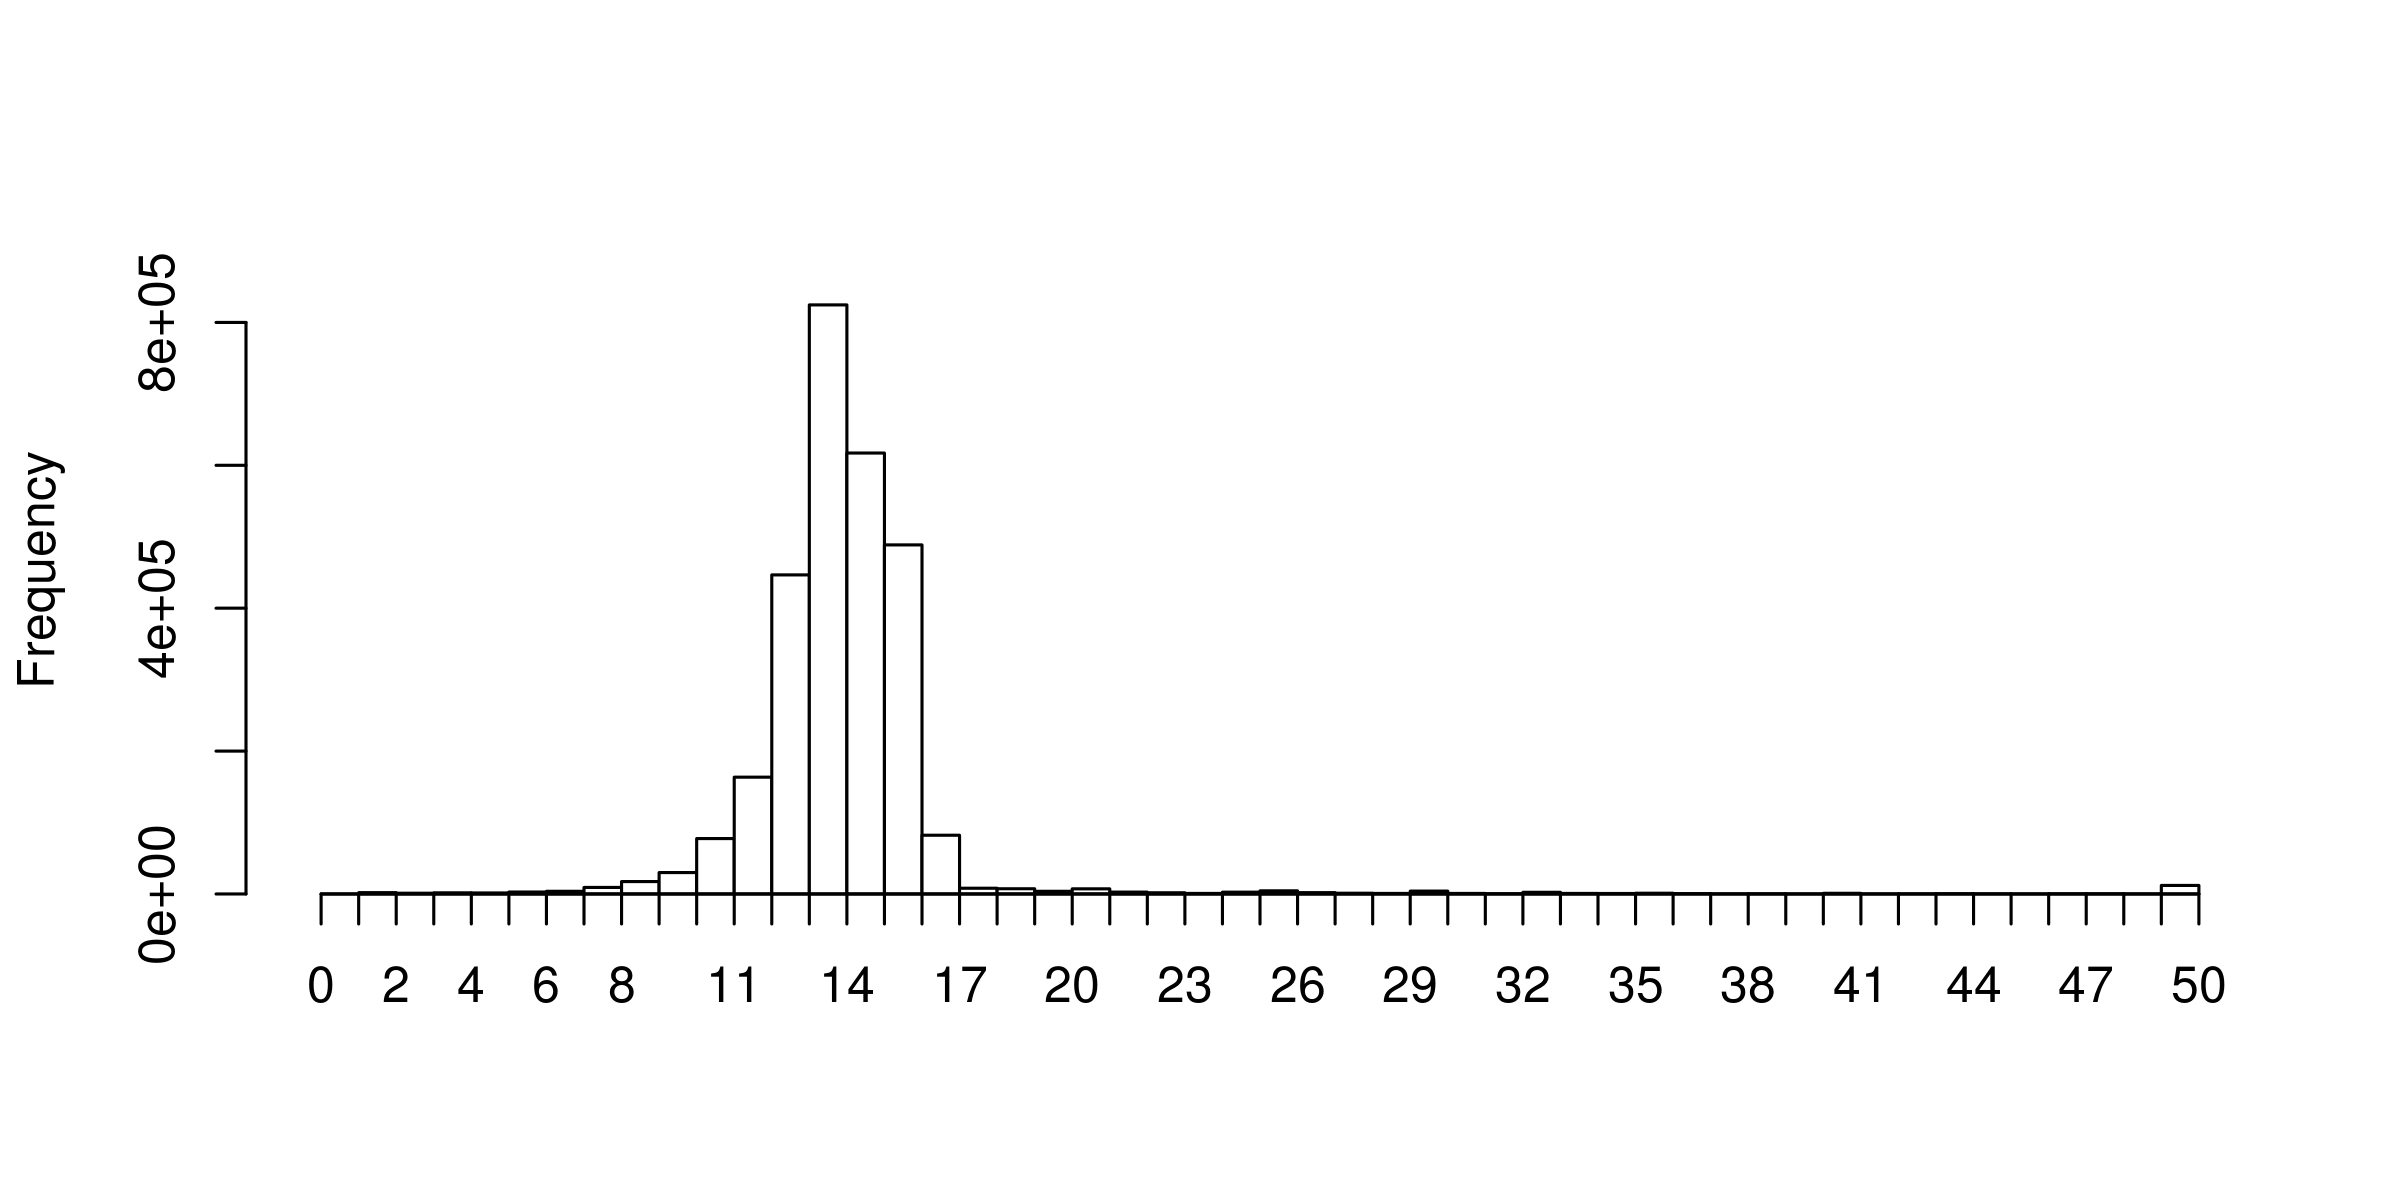
\includegraphics[width=0.8\textwidth]{de_novo/velvet/velvet_Rplot001.png}
\caption{\label{fig:SRS004748_coverage_hist} A weighted k-mer coverage histogram of the single-end reads.}
\end{figure}

\begin{steps}
After choosing the expected coverage and the coverage cut-off, you can exit R by
typing:
\begin{lstlisting}[style=R]
q()
\end{lstlisting}
\end{steps}

\begin{steps}
The weighted histogram suggests to me that the expected coverage is around 14
and that everything below 6 is likely to be noise. Some coverage is also
represented at around 20, 30 and greater 50, which might be contamination or
repeats (depending on the dataset), but at the moment this should not worry you.
To see the improvements, rerun \texttt{velvetg} first with \texttt{-cov\_cutoff} 6 and
after checking the N50 use only / add \texttt{-exp\_cov} 14 to the command line
option. Also keep a copy of the contigs file for comparison:
\begin{lstlisting}
cd ~/NGS/velvet/part1/SRS004748
time velvetg run_25 -cov_cutoff 6

# Make a copy of the run
cp run_25/contigs.fa run_25/contigs.fa.1

time velvetg run_25 -exp_cov 14
cp run_25/contigs.fa run_25/contigs.fa.2

time velvetg run_25 -cov_cutoff 6 -exp_cov 14
cp run_25/contigs.fa run_25/contigs.fa.3
\end{lstlisting}
\end{steps}

\begin{questions}
What is the N50 with no parameter:
\begin{answer}
4,447 bp
\end{answer}

What is the N50 with \texttt{-cov\_cutoff} 6:
\begin{answer}
5,168 bp
\end{answer}

What is the N50 with \texttt{-exp\_cov} 14:
\begin{answer}
4,903 bp
\end{answer}

What is the N50 with \texttt{-cov\_cutoff} 6 \texttt{-exp\_cov} 14:
\begin{answer}
5,417 bp
\end{answer}

Did you notice a variation in the time \texttt{velvetg} took to run? If so, can you
explain why that might be?
\begin{answer}
Velvet reuses already calculated results (from PreGraph,Graph)
\end{answer}

\end{questions}

\begin{steps}
You were running \texttt{velvetg} with the \texttt{-exp\_cov} and
\texttt{-cov\_cutoff} parameters. Now try to experiment using different
cut-offs, expected parameters and also explore other settings (e.g.
\texttt{-max\_coverage}, \texttt{-max\_branch\_length}, \texttt{-unused\_reads},
\texttt{-amos\_file}, \texttt{-read\_trkg} or see \texttt{velvetg} help menu).
\end{steps}

\begin{questions}
Make some notes about the parameters you've played with and the results you
obtained.
\begin{answer}
-max\_coverage: cut-off value for the upper range (like cov\_cutoff for the lower range)\\
-max\_branch\_length: length of branch to look for bubble\\
-unused\_reads: write unused reads into file\\
-amos\_file: write AMOS message file\\
-read\_trkg: tracking read (more memory usage) - automatically on for certain operations\\
\end{answer}
\\
\\
\\
\\
\end{questions}

\subsection{AMOS Hawkeye}

The \texttt{-amos\_file} argument tells \texttt{velvetg} to output the assembly
as an AMOS message file (\texttt{*.afg}) which can then be used by tools like
Hawkeye from the AMOS suite of tools.

\begin{steps}
Lets create the AMOS message file by running \texttt{velvetg} with some
appropriate parameters:
\begin{lstlisting}
velvetg run_25 -cov_cutoff 6 -exp_cov 14 -amos_file yes
\end{lstlisting}

\begin{note}
The \texttt{-exp\_cov} argument to enable read-tracking \texttt{-read\_trkg yes} in Velvet.
Without read tracking enabled, very little read-level information can be output
to the AMOS message file. This results in a pretty useless visualisation in
Hawkeye! However, since reads are being tracked, the analysis takes longer and
uses more memory.
\end{note}

Now convert the AMOS message file \texttt{velvet\_asm.afg} into an AMOS bank
using \texttt{bank-transact} and view the assembly with AMOS Hawkeye.
\begin{lstlisting}
bank-transact -c -b run_25/velvet_asm.bnk -m run_25/velvet_asm.afg
hawkeye run_25/velvet_asm.bnk
\end{lstlisting}

Have a look around the interface, in particular try to look at the ``Scaffold
View'' and ``Contig View'' of the larges scaffold. You should see something like
this:

\begin{figure}[H]
\centering
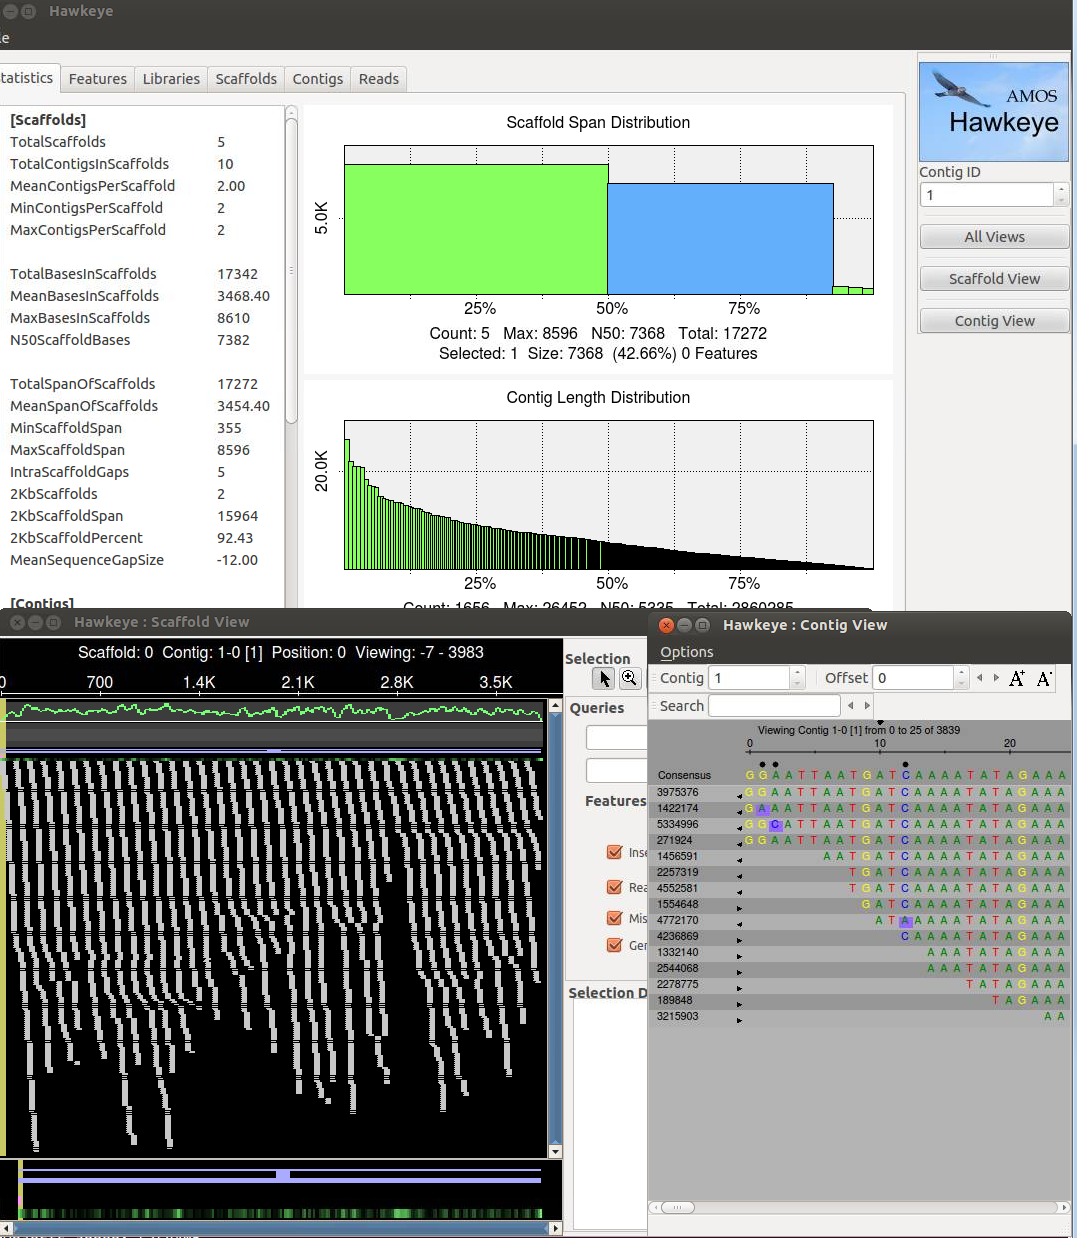
\includegraphics[width=0.8\textwidth]{de_novo/velvet/hawkeye_single_ended.png}
\caption{\label{fig:hawkeye_single_ended}}
\end{figure}

\end{steps}

\begin{bonus}
If you have time, try running the \texttt{velvetg} command without the
\texttt{-exp\_cov} argument, create the AMOS bank and see how the assemblies
look different in Hawkeye. Here's a hint:
\begin{lstlisting}
velvetg run_25 -cov_cutoff 6 -amos_file yes
bank-transact -c -b run_25/velvet_asm.bnk -m run_25/velvet_asm.afg
hawkeye run_25/velvet_asm.bnk
\end{lstlisting}

\end{bonus}

\begin{advanced}
\subsection{Simple Assembly Simulation}

\begin{note}
The data for this section is from Staphylococcus aureus MRSA252, a genome
closely related to the genome that provided the short read data in the earlier
sections of this exercise. The sequence data this time is the fully assembled
genome. The genome size is therefore known exactly and is 2,902,619 bp.
\end{note}

\begin{information}
In this exercise you will process the single whole genome sequence with \texttt{velveth}
and \texttt{velvetg}, look at the output only and go no further. The main intent of
processing this whole genome is to compute its N50 value. This must clearly be
very close to the ideal N50 value for the short reads assembly and so aid
evaluation of that assembly.
\end{information}

\begin{steps}
To begin, move back to the main directory for this exercise, make a
sub-directory for the processing of this data and move into it. All in one go,
this would be:
\begin{lstlisting}
cd ~/NGS/velvet/part1/ 
mkdir MRSA252 
cd MRSA252
\end{lstlisting}

Next, you need to download the genome sequence from
\url{http://www.ensemblgenomes.org/} which holds five new sites, for bacteria,
protists, fungi, plants and invertebrate metazoa. You could browse for the data
you require or use the file which we have downloaded for you. For the easier of
these options, make and check a symlink to the local file and with the
commands:
\begin{lstlisting}
ln -s ~/NGS/Data/s_aureus_mrsa252.EB1_s_aureus_mrsa252.dna.chromosome.Chromosome.fa.gz ./
ls -l
\end{lstlisting}

\end{steps}

\begin{note}
Usually Velvet expects relatively short sequence entries and for this reason has
a read limit of 32,767 bp per sequence entry. As the genome size is 2,902,619 bp
- longer as the allowed limit and does not fit with the standard settings into
velvet. But like the maximum k-mer size option, you can tell Velvet during
compile time, using \texttt{LONGSEQUENCES=Y}, to expect longer input sequences
than usual. I already prepared the executable which you can use by typing
\texttt{velveth\_long} and \texttt{velvetg\_long}.
\end{note}

\begin{steps}
Now, run \texttt{velveth\_long}, using the file you either just downloaded or created a
symlink to as the input:
\begin{lstlisting}
velveth_long run_25 25 -fasta.gz -long s_aureus_mrsa252.EB1_s_aureus_mrsa252.dna.chromosome.Chromosome.fa.gz
velvetg_long run_25
\end{lstlisting}

\end{steps}

\begin{questions}
What is the N50?
\begin{answer}
24,142 bp
\end{answer}

How does the N50 compare to the previous single end run (SRS004748)?
\begin{answer}
Big difference
\end{answer}
  
Does the total length differ from the input sequence length?
\begin{answer}
2,817,181 (stats) vs 2,902,619 (input)
\end{answer}
  
What happens when you rerun velvet with a different k-mer length?
\begin{answer}
K-mer 31: N50: 30,669 bp, total 2,822,878
\end{answer}

\end{questions}
\end{advanced}


\section{Assembling Paired-end Reads}

The use of paired-end data in \textit{de novo} genome assembly results in better
quality assemblies, particularly for larger, more complex genomes. In addition,
paired-end constraint violation (expected distance and orientation of paired
reads) can be used to identify misassemblies.

\begin{warning}
If you are doing \textit{de novo} assembly, pay the extra and get paired-ends:
they're worth it!
\end{warning}

\begin{note}
The data you will examine in this exercise is again from Staphylococcus aureus
which has a genome of around 3MBases. The reads are Illumina paired end with an
insert size of $~$350 bp.

The required data can be downloaded from the SRA. Specifically, the run data
(SRR022852) from the SRA Sample SRS004748.

\center{\url{http://www.ebi.ac.uk/ena/data/view/SRS004748}}

\end{note}

\begin{information}
The following exercise focuses on preparing the paired-end FASTQ files ready for
Velvet, using Velvet in paired-end mode and comparing results with Velvet's
'auto' option.
\end{information}

\begin{steps}
First move to the directory you made for this exercise and make a suitable named
directory for the exercise:
\begin{lstlisting}
cd ~/NGS/velvet/part2 
mkdir SRS004748 
cd SRS004748
\end{lstlisting}

There is no need to download the read files, as they are already stored
locally. You will simply create a symlink to this pre-downloaded data using
the following commands:
\begin{lstlisting}
ln -s ~/NGS/Data/SRR022852_?.fastq.gz ./
\end{lstlisting}

It is interesting to monitor the computer's resource utilisation, particularly
memory. A simple way to do this is to open a second terminal and in it type:
\begin{lstlisting}
top
\end{lstlisting}
\end{steps}

\begin{note}
\texttt{top} is a program that continually monitors all the processes running on
your computer, showing the resources used by each. Leave this running and refer
to it periodically throughout your Velvet analyses. Particularly if they are
taking a long time or whenever your curiosity gets the better of you. You should
find that as this practical progresses, memory usage will increase
significantly.

Now, back to the first terminal, you are ready to run \texttt{velveth} and
\texttt{velvetg}. The reads are \texttt{-shortPaired} and for the
first run you should not use any parameters for \texttt{velvetg}.
\end{note}

\begin{information}
From this point on, where it will be informative to time
your runs. This is very easy to do, just prefix the command to run the program
with the command \texttt{time}. This will cause UNIX to report how long the program took
to complete its task.
\end{information}

\begin{steps}
Set the two stages of velvet running, whilst you watch the memory usage as
reported by \texttt{top}. Time the \texttt{velvetg} stage:
\begin{lstlisting}
velveth run_25 25 -fmtAuto -create_binary -shortPaired -separate SRR022852_1.fastq.gz SRR022852_2.fastq.gz
time velvetg run_25
\end{lstlisting}

\end{steps}

\begin{questions}
What does \texttt{-fmtAuto} and \texttt{-create\_binary} do? (see help menu)
\begin{answer}
\texttt{-fmtAuto} tries to detect the correct format of the input files e.g.
  FASTA, FASTQ and whether they are compressed or not.

\texttt{-create\_binary} outputs sequences as a binary file. That means that
  \texttt{velvetg} can read the sequences from the binary file more quickly that
  from the original sequence files.
\end{answer}

Comment on the use of memory and CPU for \texttt{velveth} and \texttt{velvetg}?
\begin{answer}
\texttt{velveth} uses only one CPU while \texttt{velvetg} uses all possible CPUs
for some parts of the calculation.
\end{answer}
 
How long did \texttt{velvetg} take?
\begin{answer}
My own measurements are:\\
\texttt{real    1m8.877s; user    4m15.324s; sys     0m4.716s}
\end{answer}

\end{questions}

\begin{steps}
Next, after saving your \texttt{contigs.fa} file from being overwritten, set the
cut-off parameters that you investigated in the previous exercise and rerun
\texttt{velvetg}.
time and monitor the use of resources as previously. Start with
\texttt{-cov\_cutoff 16} thus:
\begin{lstlisting}
mv run_25/contigs.fa run_25/contigs.fa.0
time velvetg run_25 -cov_cutoff 16
\end{lstlisting}

Up until now, \texttt{velvetg} has ignored the paired-end information. Now try
running \texttt{velvetg} with both \texttt{-cov\_cutoff 16} and
\texttt{-exp\_cov 26}, but first save your \texttt{contigs.fa} file. By using
\texttt{-cov\_cutoff} and \texttt{-exp\_cov}, \texttt{velvetg} tries to estimate
the insert length, which you will see in the \texttt{velvetg} output. The
command is, of course:
\begin{lstlisting}
mv run_25/contigs.fa run_25/contigs.fa.1
time velvetg run_25 -cov_cutoff 16 -exp_cov 26
\end{lstlisting}

\end{steps}

\begin{questions}
Comment on the time required, use of memory and CPU for \texttt{velvetg}?
\begin{answer}
Runtime is lower when velvet can reuse previously calculated data. By using
\texttt{-exp\_cov}, the memory usage increases.
\end{answer}

Which insert length does Velvet estimate?
\begin{answer}
Paired-end library 1 has length: 228, sample standard deviation: 26
\end{answer}

\end{questions}

\begin{steps}
Next try running \texttt{velvetg} in `paired-end mode`. This entails running \texttt{velvetg}
specifying the insert length with the parameter \texttt{-ins\_length} set to 350. Even
though velvet estimates the insert length it is always advisable to check /
provide the insert length manually as velvet can get the statistics wrong due
to noise. Just in case, save your last version of \texttt{contigs.fa}. The commands are:
\begin{lstlisting}
mv run_25/contigs.fa run_25/contigs.fa.2
time velvetg run_25 -cov_cutoff 16 -exp_cov 26 -ins_length 350
mv run_25/contigs.fa run_25/contigs.fa.3
\end{lstlisting}
\end{steps}

\begin{questions}
How fast was this run?
\begin{answer}
My own measurements are:\\
\texttt{real    0m29.792s; user    1m4.372s; sys     0m3.880s}
\end{answer}

\end{questions}

\begin{steps}
Take a look into the Log file.
\end{steps}

\begin{questions}
What is the N50 value for the \texttt{velvetg} runs using the switches:\\
\begin{answer}
Base run: 19,510 bp
\end{answer}
\texttt{-cov\_cutoff 16}
\begin{answer}
24,739 bp
\end{answer}

\texttt{-cov\_cutoff 16 -exp\_cov 26}
\begin{answer}
61,793 bp
\end{answer}

\texttt{-cov\_cutoff 16 -exp\_cov 26 -ins\_length 350}
\begin{answer}
n50 of 62,740 bp; max 194,649 bp; total 2,871,093 bp
\end{answer}

\end{questions}

\begin{steps}
Try giving the \texttt{-cov\_cutoff} and/or \texttt{-exp\_cov} parameters the
value \texttt{auto}. See the \texttt{velvetg} help to show you how. The
information Velvet prints during running includes information about the values
used (coverage cut-off or insert length) when using the \texttt{auto} option.
\end{steps}

\begin{questions}
What coverage values does Velvet choose (hint: look at the output that Velvet
produces while running)?
\begin{answer}
Median coverage depth = 26.021837\\
Removing contigs with coverage $<$ 13.010918 \ldots
\end{answer}

How does the N50 value change?
\begin{answer}
n50 of 68,843 bp; max 194,645 bp; total 2,872,678 bp
\end{answer}
\end{questions}

\begin{steps}
Run \texttt{gnx} on all the \texttt{contig.fa} files you have generated in the
course of this exercise. The command will be:
\begin{lstlisting}
gnx -min 100 -nx 25,50,75 run_25/contigs.fa*
\end{lstlisting}
\end{steps}

\begin{questions}
For which runs are there Ns in the \texttt{contigs.fa} file and why? 
\begin{answer}
contigs.fa.2, contigs.fa.3, contigs.fa\\
Velvet tries to use the provided (or infers) the insert length and fills
ambiguous regions with Ns.
\end{answer}

Comment on the number of contigs and total length generated for each run.
\begin{answer}
\begin{table}[H]
  %\centering
    \begin{tabular}{llll}
    \toprule
    Filename & No. contigs & Total length & No. Ns \\
    \midrule
    Contigs.fa.0 & 631 & 2,830,659 & 0 \\
    Contigs.fa.1 & 580 & 2,832,670 & 0 \\
    Contigs.fa.2 & 166 & 2,849,919 & 4,847 \\
    Contigs.fa.3 & 166 & 2,856,795 & 11,713 \\
    Contigs.fa & 163 & 2,857,439 & 11,526 \\
    \bottomrule
    \end{tabular}%
  \caption{\label{tab:velvetrunresults}}%
\end{table}%
\end{answer}
\end{questions}

\subsection{AMOS Hawkeye}

We will now output the assembly in the AMOS massage format and visualise the
assembly using AMOS Hawkeye.

\begin{steps}
Run \texttt{velvetg} with appropriate arguments and output the AMOS message
file, then convert it to an AMOS bank and open it in Hawkeye:
\begin{lstlisting}
time velvetg run_25 -cov_cutoff 16 -exp_cov 26 -ins_length 350 -amos_file yes -read_trkg yes 
time bank-transact -c -b run_25/velvet_asm.bnk -m run_25/velvet_asm.afg         
hawkeye run_25/velvet_asm.bnk
\end{lstlisting}
\end{steps}

\begin{questions}
Looking at the scaffold view of a contig, comment on the proportion of ``happy
mates'' to ``compressed mates'' and ``stretched mates''.
\begin{answer}
Nearly all mates are compressed with no stretched mates and very few happy
mates.
\end{answer}

What is the mean and standard deviation of the insert size reported under the
Libraries tab?
\begin{answer}
Mean: 350 bp
SD: 35 bp
\end{answer}

Look at the actual distribution of insert sizes for this library. Can you
explain where there is a difference between the mean and SD reported in those
two places?
\begin{answer}
We specified \texttt{-ins\_length 350} to the \texttt{velvetg} command. Velvet
uses this value, in the AMOS message file that it outputs, rather than its own
estimate.
\end{answer}
\end{questions}

\begin{steps}
You can get AMOS to re-estimate the mean and SD of insert sizes using
intra-contig pairs. First, close Hawkeye and then run the following commands
before reopening the AMOS bank to see what has changed.
\begin{lstlisting}
asmQC -b run_25/velvet_asm.bnk -scaff -recompute -update -numsd 2
hawkeye run_25/velvet_asm.bnk
\end{lstlisting}
\end{steps}

\begin{questions}
Looking at the scaffold view of a contig, comment on the proportion of ``happy
mates'' to ``compressed mates'' and ``stretched mates''.
\begin{answer}
There are only a few compressed and stretched mates compared to happy mates.
There are similar numbers of stretched and compressed mates.
\end{answer}

What is the mean and standard deviation of the insert size reported under the
Libraries tab?
\begin{answer}
TODO
Mean: 226 bp
SD: 25 bp
\end{answer}

Look at the actual distribution of insert sizes for this library. Does the mean
and SD reported in both places now match?
\begin{answer}
Yes
\end{answer}

Can you find a region with an unusually high proportion of stretched, compressed,
incorrectly orientated or linking mates? What might this situation indicate?
\begin{answer}
This would indicate a possible misassembly and worthy of further investigation.

Look at the largest scaffold, there are stacks of stretched pairs which span
contig boundaries. This indicates that the gap size has been underestimated
during the scaffolding phase.
\end{answer}
\end{questions}


\subsection{Velvet and Data Quality}
So far we have used the raw read data without performing any quality control or
read trimming prior to doing our velvet assemblies.

\begin{warning}
Velvet does not use quality information present in FASTQ files.
\end{warning}

For this reason, it is vitally important to perform read QC and quality
trimming. In doing so, we remove errors/noise from the dataset which in turn
means velvet will run faster, will use less memory and will produce a better
assembly. Assuming we haven't compromised too much on coverage.

\begin{information}
To investigate the effect of data quality, we will use the run data (SRR023408)
from the SRA experiment SRX008042. The reads are Illumina paired end with an
insert size of 92 bp.
\end{information}

\begin{steps}
Go back to the main directory for this exercise and create and enter a new
directory dedicated to this phase of the exercise. The commands are:
\begin{lstlisting}
cd ~/NGS/velvet/part2 
mkdir SRX008042 
cd SRX008042
\end{lstlisting}

Create symlinks to the read data files that we downloaded for you from the SRA:
\begin{lstlisting}
ln -s ~/NGS/Data/SRR023408_?.fastq.gz ./
\end{lstlisting}
\end{steps}

\begin{note}
We will use FastQC, a tool you should be familiar with, to visualise the quality
of our data. We will use FastQC in the Graphical User Interface (GUI) mode.
\end{note}

\begin{steps}
Start FastQC and set the process running in the background, by using a trailing
\texttt{\&}, so we get control of our terminal back for entering more commands:
\begin{lstlisting}
fastqc &
\end{lstlisting}
\end{steps}

\begin{steps}
Open the two compressed FASTQ files (File $->$ Open) by selecting them both and clicking OK).
Look at tabs for both files:
\end{steps}

\begin{figure}[H]
\centering
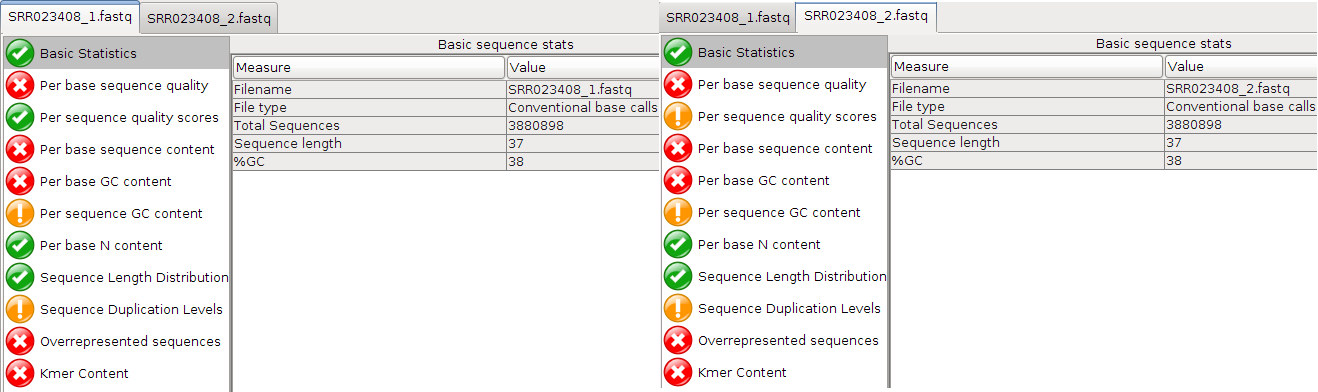
\includegraphics[width=0.8\textwidth]{de_novo/velvet/paired_fastqc.png}
\caption{\label{fig:paired_fastqc}}
\end{figure}

\begin{questions}
Are the quality scores the same for both files?
\begin{answer}
Overall yes
\end{answer}

Which value varies?
\begin{answer}
Per sequence quality scores
\end{answer}

Take a look at the Per base sequence quality for both files. Did you note that
it is not good for either file?
\begin{answer}
The quality score of both files drop very fast. Qualities of the REV strand drop
faster than the FWD strand. This is because the template has been sat around
while the FWD strand was sequenced.
\end{answer}

At which positions would you cut the reads if we did ``fixed length trimming''?
\begin{answer}
Looking at the ``Per base quality" and ``Per base sequence content'', I would
choose around 27
\end{answer}

Why does the quality deteriorate towards the end of the read?
\begin{answer}
Errors more likely for later cycles
\end{answer}

Does it make sense to trim the 5' start of reads?
\begin{answer}
Looking at the ``Per base sequence content", yes - there is a clear signal at the beginning.
\end{answer}
\end{questions}

\begin{steps}
Have a look at the other options that FastQC offers.
\end{steps}

\begin{questions}
Which other statistics could you use to support your trimming strategy?
\begin{answer}
``Per base sequence content", ``Per base GC content", ``Kmer content", ``Per
base sequence quality"
\end{answer}
\end{questions}

\begin{figure}[H]
\centering
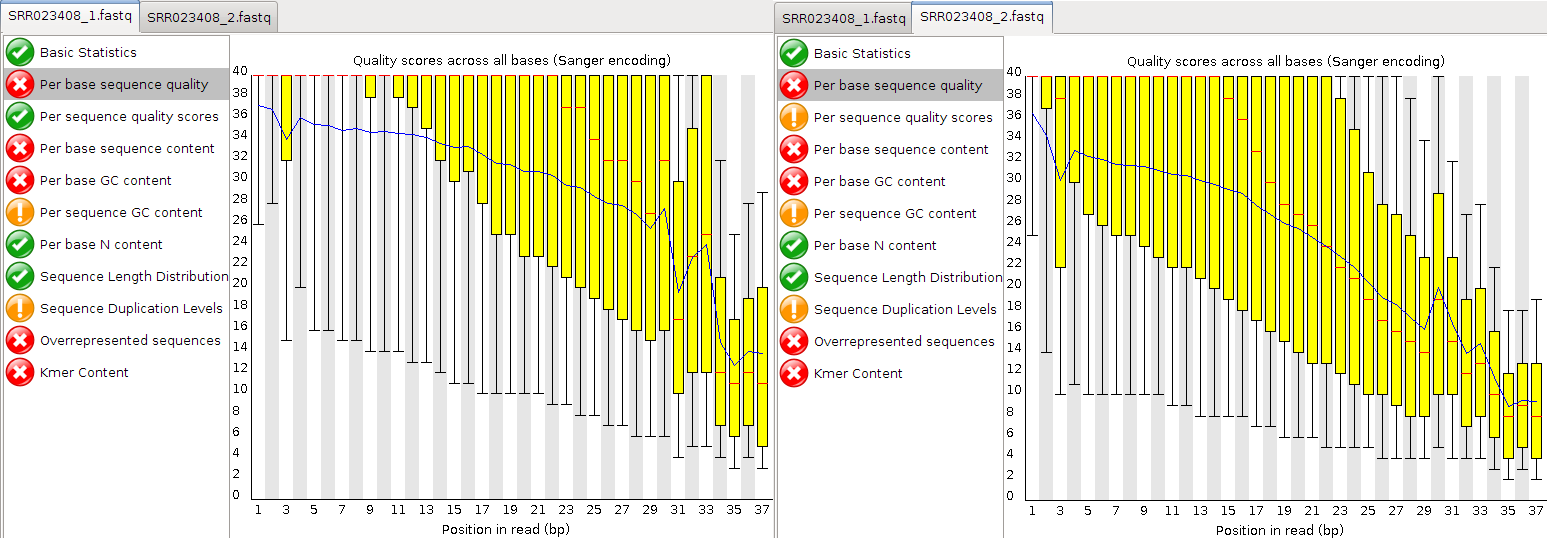
\includegraphics[width=0.8\textwidth]{de_novo/velvet/paired_fastqc_quality_plots.png}
\caption{\label{fig:paired_fastqc_quality_plots}}
\end{figure}

\begin{steps}
Once you have decided what your trim points will be, close FastQC.
We will use \texttt{fastx\_trimmer} from the FASTX-Toolkit to perform
fixed-length trimming. For usage information see the help:
\begin{lstlisting}
fastx_trimmer -h
\end{lstlisting}

\begin{note}
\texttt{fastx\_trimmer} is not able to read compressed FASTQ files, so we first
need to decompress the files ready for input.
\end{note}

The suggestion (hopefully not far from your own thoughts?) is that you trim your
reads as follows:

\begin{lstlisting}
gunzip < SRR023408_1.fastq.gz > SRR023408_1.fastq
gunzip < SRR023408_2.fastq.gz > SRR023408_2.fastq
fastx_trimmer -Q 33 -f 1 -l 32 -i SRR023408_1.fastq -o SRR023408_trim1.fastq 
fastx_trimmer -Q 33 -f 1 -l 27 -i SRR023408_2.fastq -o SRR023408_trim2.fastq
\end{lstlisting}

\begin{advanced}
Many NGS read files are large. This means that simply reading and writing files
can become the bottleneck, also known as I/O bound. Therefore, it is often good practice to
avoid unnecessary disk read/write.

We could do what is called pipelining to send a stream of data from one command
to another, using the pipe (\texttt{|}) character, without the need for
intermediary files. The following command would achieve this:
\begin{lstlisting}
gunzip --to-stdout < SRR023408_1.fastq.gz | fastx_trimmer -Q 33 -f 4 -l 32 -o SRR023408_trim1.fastq 
gunzip --to-stdout < SRR023408_2.fastq.gz | fastx_trimmer -Q 33 -f 3 -l 29 -o SRR023408_trim2.fastq
\end{lstlisting}
\end{advanced}

Now run \texttt{velveth} with a k-mer value of 21 for both the untrimmed and
trimmed read files in \texttt{-shortPaired} mode. Separate the output of the two
executions of \texttt{velveth} into suitably named directories, followed by
\texttt{velvetg}:
\begin{lstlisting}
# untrimmed reads
velveth run_21 21 -fmtAuto -create_binary -shortPaired -separate SRR023408_1.fastq SRR023408_2.fastq
time velvetg run_21

# trimmed reads
velveth run_21trim 21 -fmtAuto -create_binary -shortPaired -separate SRR023408_trim1.fastq SRR023408_trim2.fastq
time velvetg run_21trim
\end{lstlisting}
\end{steps}

\begin{questions}
How long did the two \texttt{velvetg} runs take?
\begin{answer}
run\_25:      \texttt{real    3m16.132s; user    8m18.261s; sys     0m7.317s}\\
run\_25trim:  \texttt{real    1m18.611s; user    3m53.140s; sys     0m4.962s}
\end{answer}

What N50 scores did you achieve?
\begin{answer}
Untrimmed: 11\\
Trimmed: 15
\end{answer}

What were the overall effects of trimming?
\begin{answer}
Time saving, increased N50, reduced coverage
\end{answer}
\end{questions}

\begin{steps}
The evidence is that trimming improved the assembly. The thing to do surely, is
to run \texttt{velvetg} with the \texttt{-cov\_cutoff} and \texttt{-exp\_cov}. In order
to use \texttt{-cov\_cutoff} and \texttt{-exp\_cov} sensibly, you need to
investigate with R, as you did in the previous exercise, what parameter values
to use. Start up R and produce the weighted histograms:
\begin{lstlisting}[style=R]
R --no-save
library(plotrix) 
data <- read.table("run_21/stats.txt", header=TRUE) 
data2 <- read.table("run_21trim/stats.txt", header=TRUE) 
par(mfrow=c(1,2))
weighted.hist(data$short1_cov, data$lgth, breaks=0:50)
weighted.hist(data2$short1_cov, data2$lgth, breaks=0:50)
\end{lstlisting}

\begin{figure}[H]
\centering
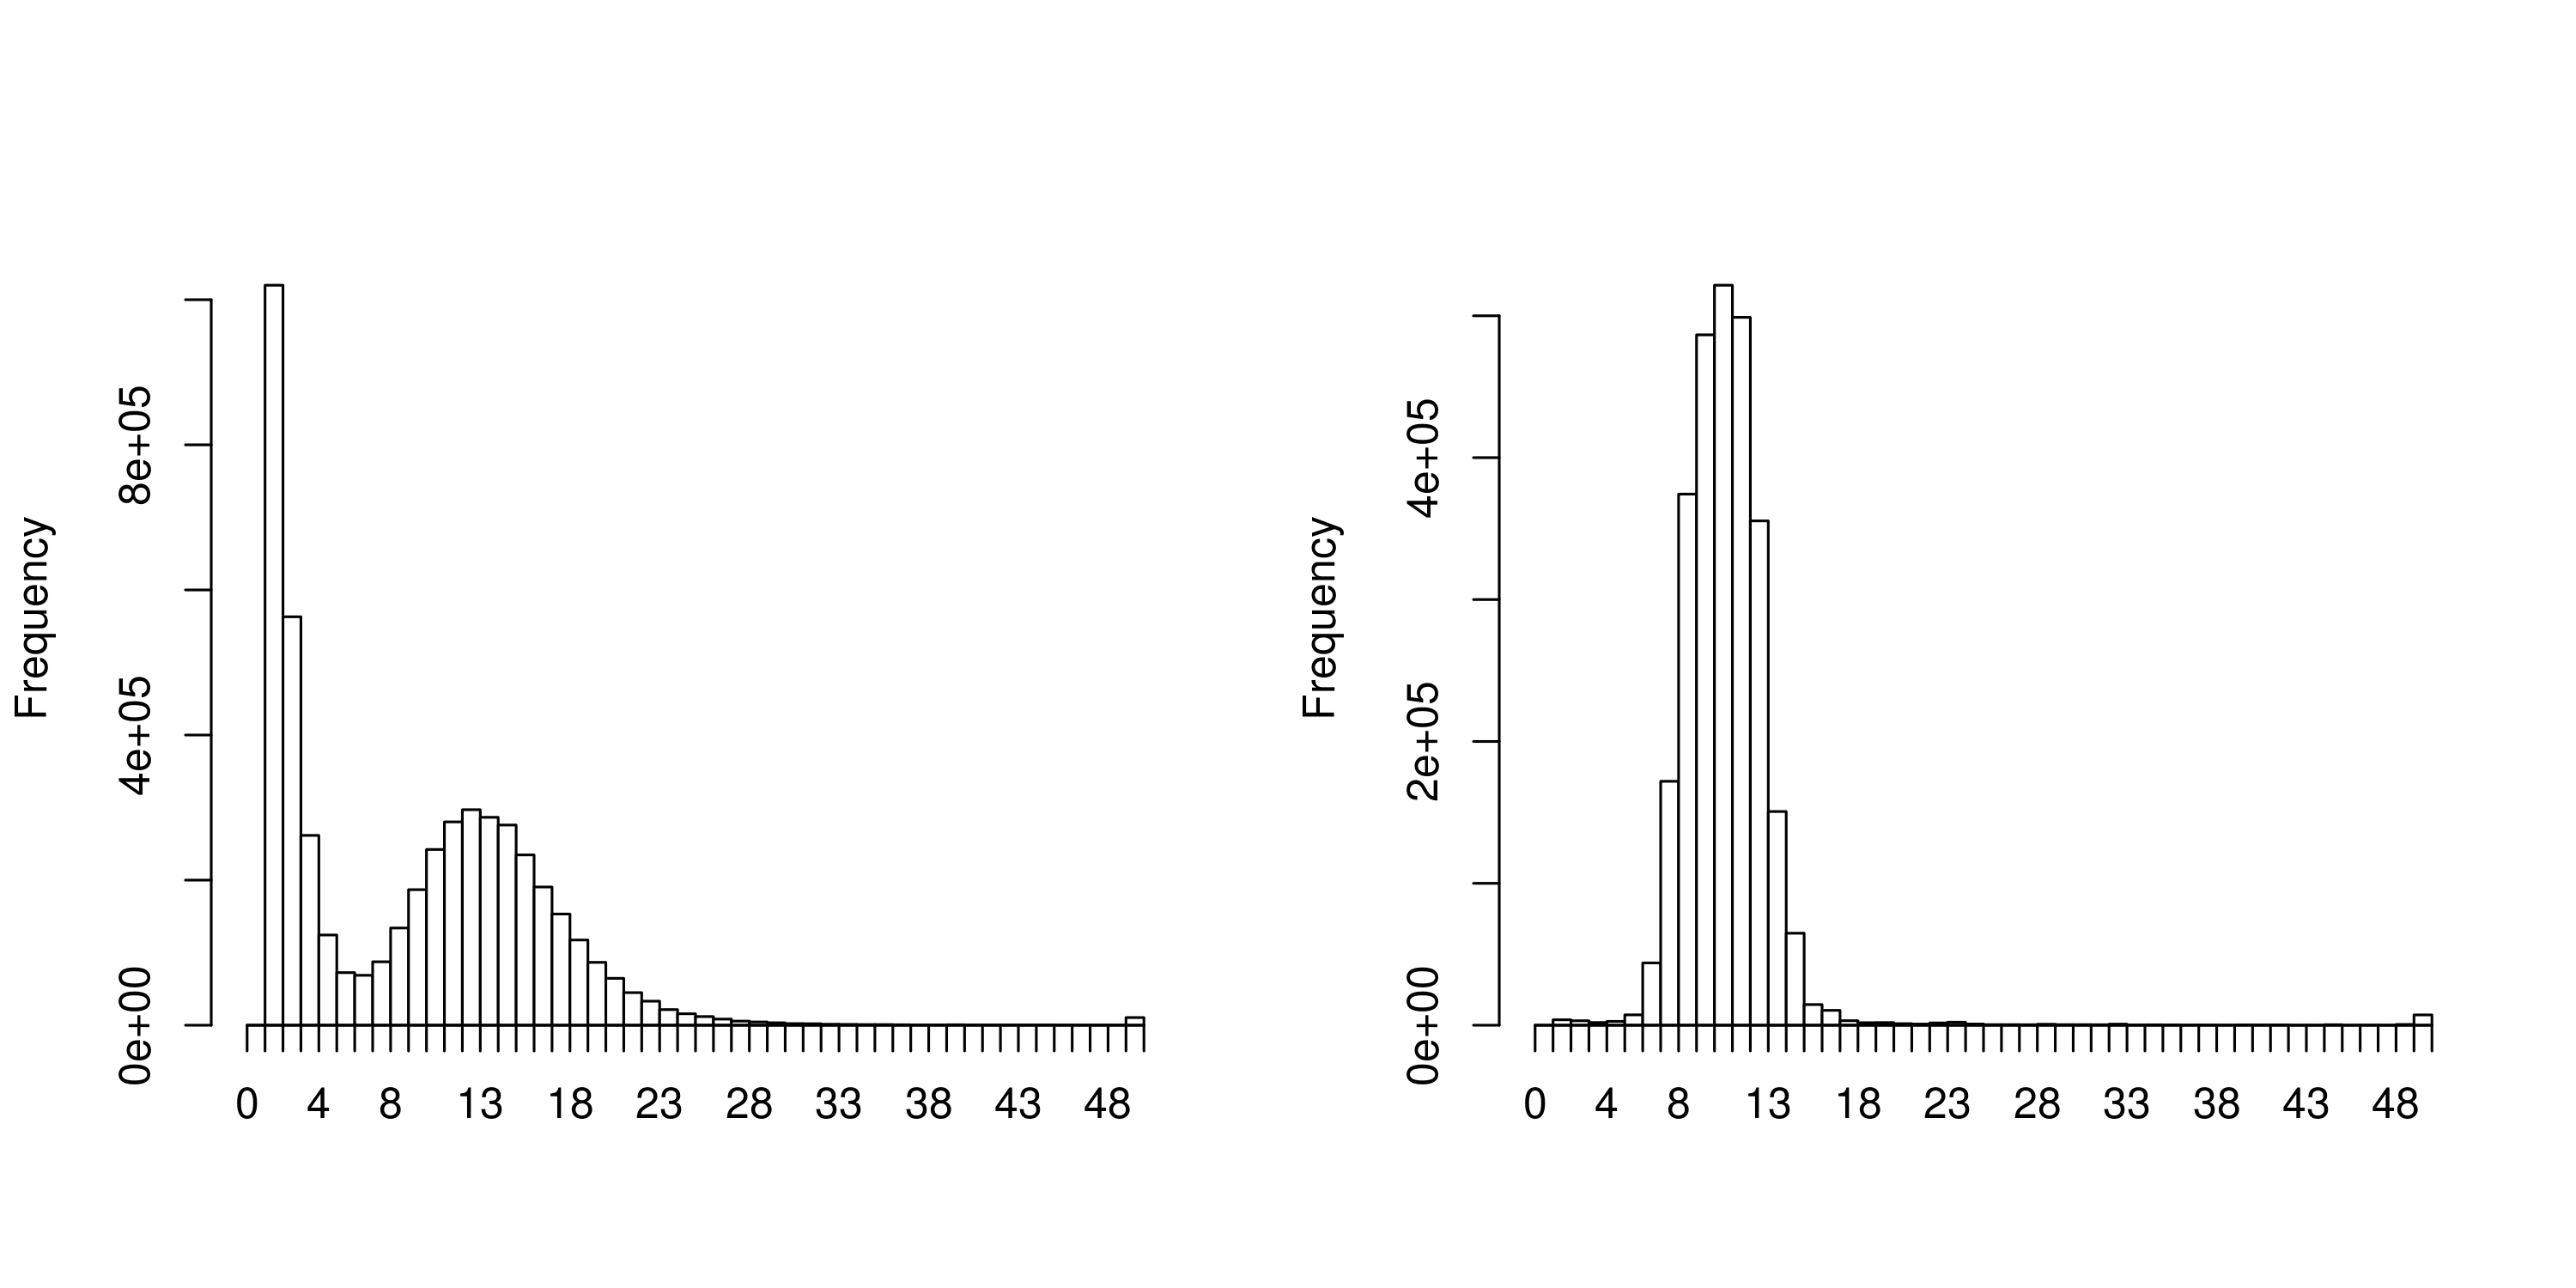
\includegraphics[width=0.8\textwidth]{de_novo/velvet/velvet_Rplot002.png}
\caption{\label{fig:velvet_Rplot002} Weighted k-mer coverage histograms of the paired-end reads pre-trimmed (left) and post-trimmed (right).}
\end{figure}

For the untrimmed read histogram (left) there is an expected coverage of around
13 with a coverage cut-off of around 7. For the trimmed read histogram (right)
there is an expected coverage of around 9 with a coverage cut-off of around 5.

If you disagree, feel free to try different settings, but first quit R before
running \texttt{velvetg}:
\begin{lstlisting}[style=R]
q()
\end{lstlisting}

\begin{lstlisting}
time velvetg run_21 -cov_cutoff 7 -exp_cov 13 -ins_length 92
time velvetg run_21trim -cov_cutoff 5 -exp_cov 9 -ins_length 92
\end{lstlisting}

\end{steps}

\begin{questions}
How good does it look now?\\
\begin{answer}
Still not great
\end{answer}
Comment on:\\ 
Runtime
\begin{answer}
Reduced runtime
\end{answer}

Memory
\begin{answer}
Lower memory usage
\end{answer}

k-mer choice (Can you use k-mer 31 for a read of length 30 bp?)
\begin{answer}
K-mer has to be lower than the read length and the K-mer coverage should be
sufficient to produce results.
\end{answer}

Does less data mean ``worse" results?
\begin{answer}
Not necessarily. If you have lots of data you can safely remove poor data
without too much impact on overall coverage.
\end{answer}
  
How would a smaller/larger k-mer size behave?
\begin{answer}
% TODO
\end{answer}
\end{questions}

\begin{steps}
Compare the results, produced during the last exercises, with each other:

\begin{table}[H]
  \centering
    \begin{tabular*}{0.9\textwidth}{l|l|l|l}
    \toprule
    Metric & SRR022852 & SRR023408 & SRR023408.trimmed \\
    \midrule
    Overall Quality (1-5) & & & \\[0.5\questionspacing]
    \hline
    bp Coverage & & & \\[0.5\questionspacing]
    \hline
    k-mer Coverage & & & \\[0.5\questionspacing]
    \hline
    N50 (k-mer used) & & & \\[0.5\questionspacing]
    \bottomrule
    \end{tabular*}
  \caption{\label{tab:comparison}}
\end{table}

\begin{answer}
\begin{table}[H]
  \centering
    \begin{tabular*}{0.9\textwidth}{l|l|l|l}
    \toprule
    Metric & SRR022852 & SRR023408 & SRR023408.trimmed \\
    \midrule
    Overall Quality (1-5) & 2 & 5 & 4\\[0.5\questionspacing]
    \hline
    bp Coverage & 136 x (36 bp;11,374,488) & 95x (37bp; 7761796) & 82x (32bp; 7761796)\\[0.5\questionspacing]
    \hline
    k-mer Coverage & 45x & 43x (21); 33x (25) & 30x (21); 20.5x (25)\\[0.5\questionspacing]
    \hline
    N50 (k-mer used) & 68,843 (25) & 2,803 (21) & 2,914 (21)\\[0.5\questionspacing]
    \bottomrule
    \end{tabular*}
  \caption{\label{tab:comparison_result}}
\end{table}
\end{answer}

\end{steps}

\begin{questions}
What would you consider as the ``best" assembly?
\begin{answer}
SRR022852
\end{answer}

If you found a candidate, why do you consider it as ``best" assembly?
\begin{answer}
Overall data quality and coverage
\end{answer}

How else might you assess the the quality of an assembly? Hint: Hawkeye.
\begin{answer}
By trying to identify paired-end constraint violations using AMOS Hawkeye.
\end{answer}
\end{questions}


%\section{Assembling Long (454) Read}

\begin{note}
The data you will examine in this exercise is again from Staphylococcus aureus
which has a genome of around 3MB. The reads are 454 single end.

The required data can be downloaded from the SRA. Specifically, the run data
(SRR000892, SRR000893) from the SRA Experiment SRX000181.

\center{\url{http://www.ebi.ac.uk/ena/data/view/SRX000181}}
\end{note}

\begin{information}
The following exercise focuses on processing 454 long reads with velvet and how
this differs compared to short reads.
\end{information}

\begin{steps}
First move to the directory you made for this exercise and make a suitable named
directory for the exercise before downloading the read files:
\begin{lstlisting}
cd ~/NGS/velvet/part3
mkdir SRX000181
cd SRX000181
\end{lstlisting}

The downloaded files can be used directly in velvet. To let velvet know that
these FASTQ files are long reads, you pass in the parameter \texttt{-long} by
using the commands:
\begin{lstlisting}
ln -s ~/NGS/Data/SRR000892.fastq.gz
ln -s ~/NGS/Data/SRR000893.fastq.gz
velveth run_25 25 -create_binary -fastq.gz -long *.fastq.gz
time velvetg run_25
\end{lstlisting}
\end{steps}

\begin{questions}
Take a look at the \texttt{stats.txt} file. Which columns are used compared to
short reads and why?
\begin{answer}
long\_cov instead of e.g. short1\_cov
\end{answer}

Which N50 do you get?
\begin{answer}
28 (k-mer N50)
\end{answer}

How long did the \texttt{velvetg} run take?
\begin{answer}
\texttt{real    0m36.333s; user    2m33.238s; sys     0m3.893s}
\end{answer}
\end{questions}

\begin{steps}
The right thing to do is to run \texttt{velvetg} setting the cut-offs. But for long reads
there is an option called \texttt{-long\_cov\_cutoff} to filter them
independently because of the difference in usage in velvet. To investigate with
R, as you did in the previous exercises, start up R and produce the weighted
histogram using the column \texttt{long\_cov} by typing:
\begin{lstlisting}[style=R]
R --no-save
library(plotrix) 
data <- read.table("run_25/stats.txt", header=TRUE) 
weighted.hist(data$long_cov, data$lgth, breaks=0:50)
\end{lstlisting}

\begin{figure}[H]
\centering
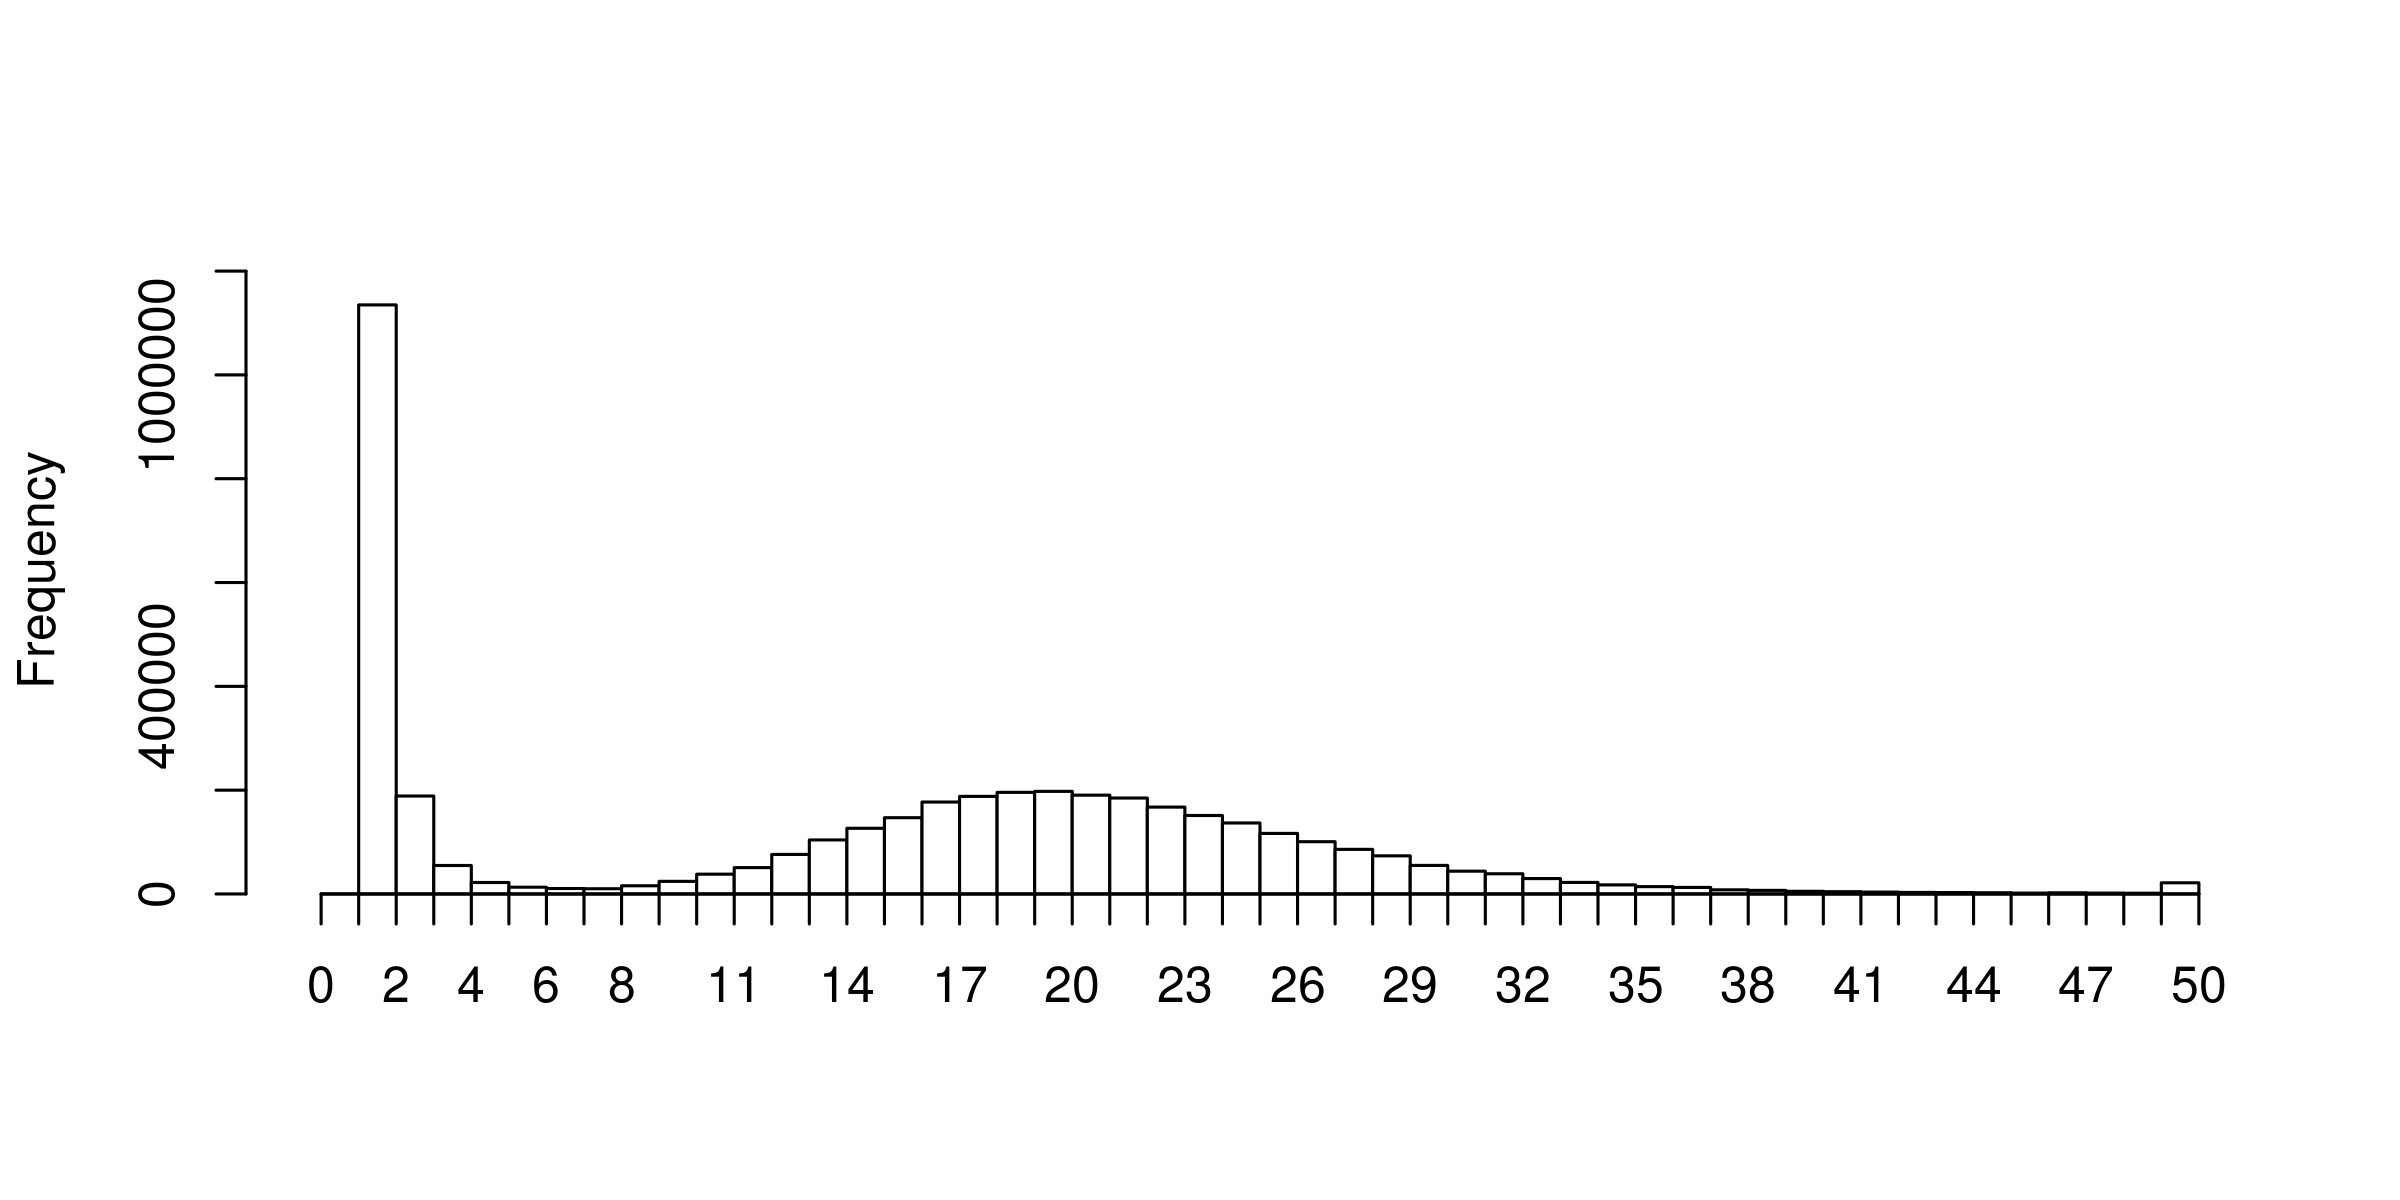
\includegraphics[width=0.8\textwidth]{de_novo/velvet/velvet_Rplot003.png}
\caption{\label{fig:velvetRplot003}}
\end{figure}

For me the histogram suggests to me to choose a coverage cut-off of around 9
with an expected coverage of about 19.

If you disagree, feel free to try different settings, but first leave R before
running \texttt{velvetg}:
\begin{lstlisting}[style=R]
q()
\end{lstlisting}

\begin{lstlisting}
cp run_25/contigs.fa run_25/contigs.fa.0

time velvetg run_25 -long_cov_cutoff 9
cp run_25/contigs.fa run_25/contigs.fa.1

time velvetg run_25 -long_cov_cutoff 9 -exp_cov 19
cp run_25/contigs.fa run_25/contigs.fa.2

gnx -min 100 -nx 25,50,75 run_25/contigs.fa*
\end{lstlisting}

\end{steps}

\begin{questions}
What is the N50 and runtime using:\\
\texttt{-long\_cov\_cutoff 9}
\begin{answer}
\texttt{5,747; real  0m11.457s; user  0m10.855s; sys  0m0.329s}
\end{answer}

\texttt{-long\_cov\_cutoff 9 -exp\_cov 19}
\begin{answer}
\texttt{16,781; real 0m29.830s; user 2m32.530s; sys 0m3.523s}
\end{answer}

other runs?

Which other parameters could improve the assembly quality for long reads?
\begin{answer}
\texttt{-conserveLong}
\end{answer}

What do you think about assembling 454 reads with Velvet?
\begin{answer}
It's working!
\end{answer}
\end{questions}


%\section{Assembling Multiple Insert Length Libraries}

\begin{note}
Like the previous examples, the data you will examine in this exercise is again
from Staphylococcus aureus which still has a genome of around 3MB. The reads are
Illumina paired end with an insert size of 170 bp and 350 bp.

You already downloaded the required reads from the SRA in previous exercises.
Specifically, the run data (SRR022863, SRR022852) from the SRA Study SRP001086.

\center{\url{http://www.ebi.ac.uk/ena/data/view/SRP001086}}
\end{note}

\begin{information}
The following exercise focuses on handing two insert length libraries with
velvet and the changes you have to look out for.
\end{information}

\begin{steps}
First move to the directory you made for this exercise, make a suitable named
directory for the exercise and check if all the files are in place:
\begin{lstlisting}
cd ~/NGS/velvet/part3
mkdir SRP001086
cd SRP001086
ln -s ~/NGS/Data/SRR022863_?.fastq.gz ./
ln -s ~/NGS/Data/SRR022852_?.fastq.gz ./
\end{lstlisting}

Now run \texttt{velveth} and \texttt{velvetg} using the appropriate command line
options by typing:
\begin{lstlisting}
time velveth run_25 25 -fmtAuto -create_binary -shortPaired -separate SRR022863_1.fastq.gz SRR022863_2.fastq.gz -shortPaired2 -separate SRR022852_1.fastq.gz SRR022852_2.fastq.gz
time velvetg run_25
\end{lstlisting}

The right thing to do is to run velvetg setting the cut-offs. To investigate
with R, as you did in the previous exercises, start up R and produce the
weighted histogram using the columns \texttt{short1\_cov} and
\texttt{short2\_cov} by typing:
\begin{lstlisting}[style=R]
R --no-save
library(plotrix) 
data <- read.table("run_25/stats.txt", header=TRUE) 
weighted.hist(data$short1_cov+data$short2_cov, data$lgth, breaks=0:70)
\end{lstlisting}

\begin{figure}[H]
\centering
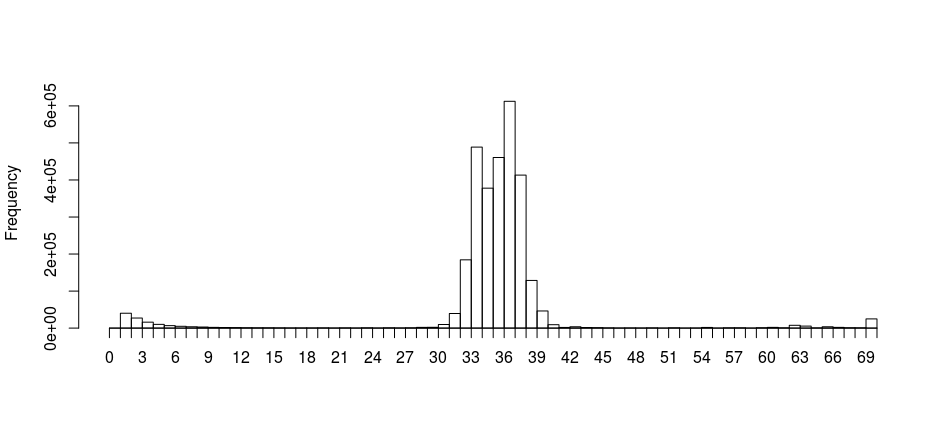
\includegraphics[width=0.8\textwidth]{de_novo/velvet/velvet_Rplot004.png}
\caption{\label{fig:velvet_Rplot004}}
\end{figure}

For me the histogram suggests a coverage cut-off of around 28
with an expected coverage of about 36. If you disagree, feel free to try
different settings, but first leave R before running \texttt{velvetg} with the coverage
parameters typing:
\begin{lstlisting}[style=R]
q()
\end{lstlisting}

\begin{lstlisting}
cp run_25/contigs.fa run_25/contigs.fa.0

time velvetg run_25 -cov_cutoff 28 
cp run_25/contigs.fa run_25/contigs.fa.1

time velvetg run_25 -cov_cutoff 28 -exp_cov 36 
cp run_25/contigs.fa run_25/contigs.fa.2

time velvetg run_25 -cov_cutoff 28 -exp_cov 36 -ins_length 170 -ins_length2 350
cp run_25/contigs.fa run_25/contigs.fa.3

gnx -min 100 -nx 25,50,75 run_25/contigs.fa*
\end{lstlisting}

\end{steps}

\begin{questions}
What was the best N50 you got?
\begin{answer}
62,741 bp
\end{answer}

How did the runtime/results compare to a run with a single paired-end library?
\begin{answer}
More memory, longer runtime, (in this case) similar results
\end{answer}

How many different libraries would you be able to run with this velvet version?
\begin{answer}
2 paired-end (or mate-pair) + one single end
\end{answer}

Would you be able to add a single-end library as well with this velvet version?
\begin{answer}
Yes
\end{answer}
\end{questions}


\begin{bonus}
Output an AMOS message file, convert it into an AMOS bank, update the
estimations for the insert size distributions and view the assembly with
Hawkeye.

\begin{lstlisting}
time velvetg run_25 -cov_cutoff 28 -exp_cov 36 -ins_length 170 -ins_length2 350 -amos_file yes -read_trkg yes
cp run_25/contigs.fa run_25/contigs.fa.4
gnx -min 100 -nx 25,50,75 run_25/contigs.fa.4

bank-transact -c -b run_25/velvet_asm.bnk -m run_25/velvet_asm.afg
asmQC -b run_25/velvet_asm.bnk -scaff -recompute -update -numsd 2
hawkeye run_25/velvet_asm.bnk
\end{lstlisting}

\begin{questions}
What are the mean and SD for the insert size distributions for the two libraries
used in the assembly?
\begin{answer}
Mean: 129; SD:31
Mean: 227; SD:19
\end{answer}
\end{questions}

\end{bonus}

% \begin{bonus}
% Find and download a different insert length library
% % TODO: \footnote affects the width of the shaded box - \renewcommand{\footnote}?
% \footnotemark[1]
% from the
% study SRP001086 and recompile velvet to allow the use of three insert length
% libraries. Maybe you could use the library you trimmed during previous
% exercises. You should be able to find these files here:
% \texttt{~/NGS/velvet/part2/SRX008042/SRR023408\_trim?.fastq}. If you don't still
% have these files, you can find a copy of them here:
% \texttt{~/NGS/Data/SRR023408\_trim?.fastq}.
% Use the fresh compiled Velvet version with the three (two provided and one
% downloaded library) to assemble the genome.
% \begin{questions}
% Does the extra library make any difference?
% \begin{answer}
% % TODO
% \end{answer}
% 
% How does the overall coverage change?
% \begin{answer}
% % TODO
% \end{answer}
% 
% Any other comments?
% \begin{answer}
% % TODO
% \end{answer}
% \end{questions}
% \footnotetext[1]{Paired insert
% lengths can be found on the NCBI SRA page in the library section (Nominal
% length) e.g. \url{http://www.ncbi.nlm.nih.gov/sra?term=SRR022866}}
% \end{bonus}


\begin{advanced}
\section{Hybrid Assembly}
\begin{note}
Like the previous examples, the data you will examine in this exercise is again
from Staphylococcus aureus which has a genome of around 3MB. The reads are 454
single end and Illumina paired end with an insert size of 170 bp.
You already downloaded the required reads from the SRA in previous exercises.
Specifically, the run data (SRR022863, SRR000892, SRR000893) from the SRA
experiments SRX007709 and SRX000181.
\end{note}

\begin{information}
The following exercise focuses on handing 454 long reads and paired-end reads
with velvet and the differences in setting parameters.
\end{information}

\begin{steps}
First move to the directory you made for this exercise, make a suitable named
directory for the exercise and check if all the three files are in place:
\begin{lstlisting}
cd ~/NGS/velvet/part3
mkdir SRR000892-SRR022863 
cd SRR000892-SRR022863
# 454 single end data
ln -s ~/NGS/Data/SRR00089[2-3].fastq.gz ./
# illumina paired end data
ln -s ~/NGS/Data/SRR022863_?.fastq.gz ./
\end{lstlisting}
\end{steps}

\begin{warning}
The following command will run for a LONG time. This indicated the amount of
calculations being preformed by Velvet to reach a conclusion. To wait for velvet
to finish would exceed the time available in this workshop, but it is up to you
to either let it run over night or kill the process by using the key combination
\texttt{CTRL+c}.
\begin{lstlisting}
velveth run_25 25 -fmtAuto -create_binary -long SRR00089?.fastq.gz -shortPaired -separate SRR022863_1.fastq.gz SRR022863_2.fastq.gz
time velvetg run_25
\end{lstlisting}

\begin{steps}
If you have decided to continue, we already inspected the weighted histograms
for the short and long read library separately, you can reuse this for the
cut-off values:
\begin{lstlisting}
time velvetg run_25 -cov_cutoff 7 -long_cov_cutoff 9
\end{lstlisting}
\end{steps}

\begin{questions}
What are your conclusions using Velvet in an hybrid assembly?
\begin{answer}
17 min:  time velvetg run\_25
\end{answer}
\end{questions}

\end{warning}
\end{advanced}

